\documentclass{article}

% packages and stuff
\usepackage[utf8]{inputenc}
\usepackage[headheight = 18pt, footskip = 10pt]{geometry}
    \geometry{a4paper}
    \geometry{left=0.5in, right=0.5in, top=.95in, bottom=.95in}
\usepackage{graphicx}
\usepackage{amsmath}
%Better boxed command in math mode
\usepackage{empheq}
%Input text files and code
\usepackage{verbatim}
%Bold math
\usepackage{bm}
%Cancel to in math mode
\usepackage{cancel}
% Input standalone tex documents
\usepackage{standalone}
\usepackage{subcaption}
\usepackage{ulem}
\usepackage{bigstrut}
\usepackage{bm}
\usepackage{multirow}
\usepackage{calc}
\usepackage{xkeyval}
\usepackage{color, soul}
\usepackage{ifthen}
\usepackage{import}
\usepackage{times}
\usepackage{longtable}
\usepackage{tabularx}
\usepackage{multicol}
\usepackage{wrapfig}
\usepackage[font={small,it}]{caption}
\usepackage[version=4]{mhchem}
\usepackage{booktabs}
\usepackage{longtable}
\usepackage{epigraph}

%New colors defined below
\definecolor{codegreen}{rgb}{0,0.6,0}
\definecolor{codegray}{rgb}{0.5,0.5,0.5}
\definecolor{codepurple}{rgb}{0.58,0,0.82}
\definecolor{backcolour}{rgb}{0.95,0.95,0.92}

% Include external pdf documents
\usepackage{pdfpages}

%Nice captions in floating figures
\usepackage{caption}

%%%%%%%%%%%%%%%%%%%%%%%%%%%%%%%%%%%%%%%%%%%%%%%%%%%%%%%%%%%%%%%%%%%%%%%%%%%%%%%%
\usepackage{fancyvrb}
\usepackage{comment}
\usepackage{enumerate}
\usepackage{subfiles}

%%%%%%%%%%%%%%%%%%%%%%%%%%%%%%%%%%%%%%%%%%%%%%%%%%%%%%%%%%%%%%%%%%%%%%%%%%%%%%%

% capital H is a champion
\usepackage{float}
    \restylefloat{table}

% make section styles non-lame
\usepackage{sectsty}
    \allsectionsfont{\mdseries\upshape}

% easy coloring for todo notes
\newcommand{\done}{\todo[inline, color=green]{(DONE)}{}}
\newcommand{\notdone}{\todo[inline, color=red]{(NOT DONE)}{}}
\newcommand{\fix}[1]{\todo[inline, color=red!75]{(FIX) #1}{}}
\newcommand{\discuss}[1]{\todo[inline, color=blue!40]{(DISCUSS) #1}{}}
\newcommand{\note}[1]{\todo[inline, color=yellow!20]{(NOTE) #1}}
\newcommand{\review}{\todo[inline, color=red!45!yellow!45]{(REVIEW)}{}}


\pagenumbering{gobble}
\setlength\parindent{10pt}
\setlength{\parskip}{0pt}
\setlength{\abovedisplayskip}{0pt}
\setlength{\belowdisplayskip}{0pt}
\relpenalty=10000 % don't split equations!!
\binoppenalty=10000 % don't split equations!!

\newcommand{\FigSiz}{0.37\textwidth}

% Set global figure size variable

\makeatletter
\define@key{Gin}{figsize}[true]{%
    \edef\@tempa{{Gin}{width=\FigSiz}}%
    \expandafter\setkeys\@tempa
}
\makeatother


%%%%%%%%%%%%%%%%%%%%%%%%%%%%%%%%%%%%%%%%%%%%%%%%%%%%%%%%%%%%%%%%%%%%%%%%%%%%%%%%%%%%%%%%%%%%%%%


% Custom title
\pagenumbering{arabic}
\usepackage{lastpage}
\usepackage{fancyhdr}
    \fancyhead{}
    \fancyfoot{}
    \pagestyle{fancy}
    \chead{\Large CS575: Project 6}
    \lhead{\Large Andrew Alferman}
    \rhead{\Large \today}
    \cfoot{\thepage  ~\ of ~\pageref{LastPage}}

\usepackage{titlesec}
\titlespacing*{\subsection}
{0pt}{0.65\baselineskip}{0.65\baselineskip}

%%%%%%%%%%%%%%%%%%%%%%%%%%%%%%%%%%%%%%%%%%%%%%%%%%%%%%%%%%%%%%%%%%%%%%%%%%%%%%%%%%%%%%%%%%%%%%%
\begin{document}



% Brief summary of the assignment
The purpose of this assignment was to ...

\subsection*{Question 1}
\textit{What machines did you run the experiment on?}

Flip was used to obtain data for serial processing, OpenMP processing, and SIMD processing on its CPU at a time when the load average was approximately XX.X.  Rabbit was used to obtain data for serial processing and OpenMP processing on its CPU, and OpenCL processing on its GPU at a time when the load average was approximately XX.X

\subsection*{Question 2}
\textit{Show the \texttt{Sums[1]} ... \texttt{Sums[512]} vs. shift scatterplot.}






Graphs of the computation speed versus the global size and local work group size can be found in Figures \ref{fig:MultGlobal} and \ref{fig:MultLocal}.  A table of the values used to generate these graphs can be found in Table \ref{tab:Data} of Appendix \ref{app:Data}.
\begin{figure}[h!]
	\centering
        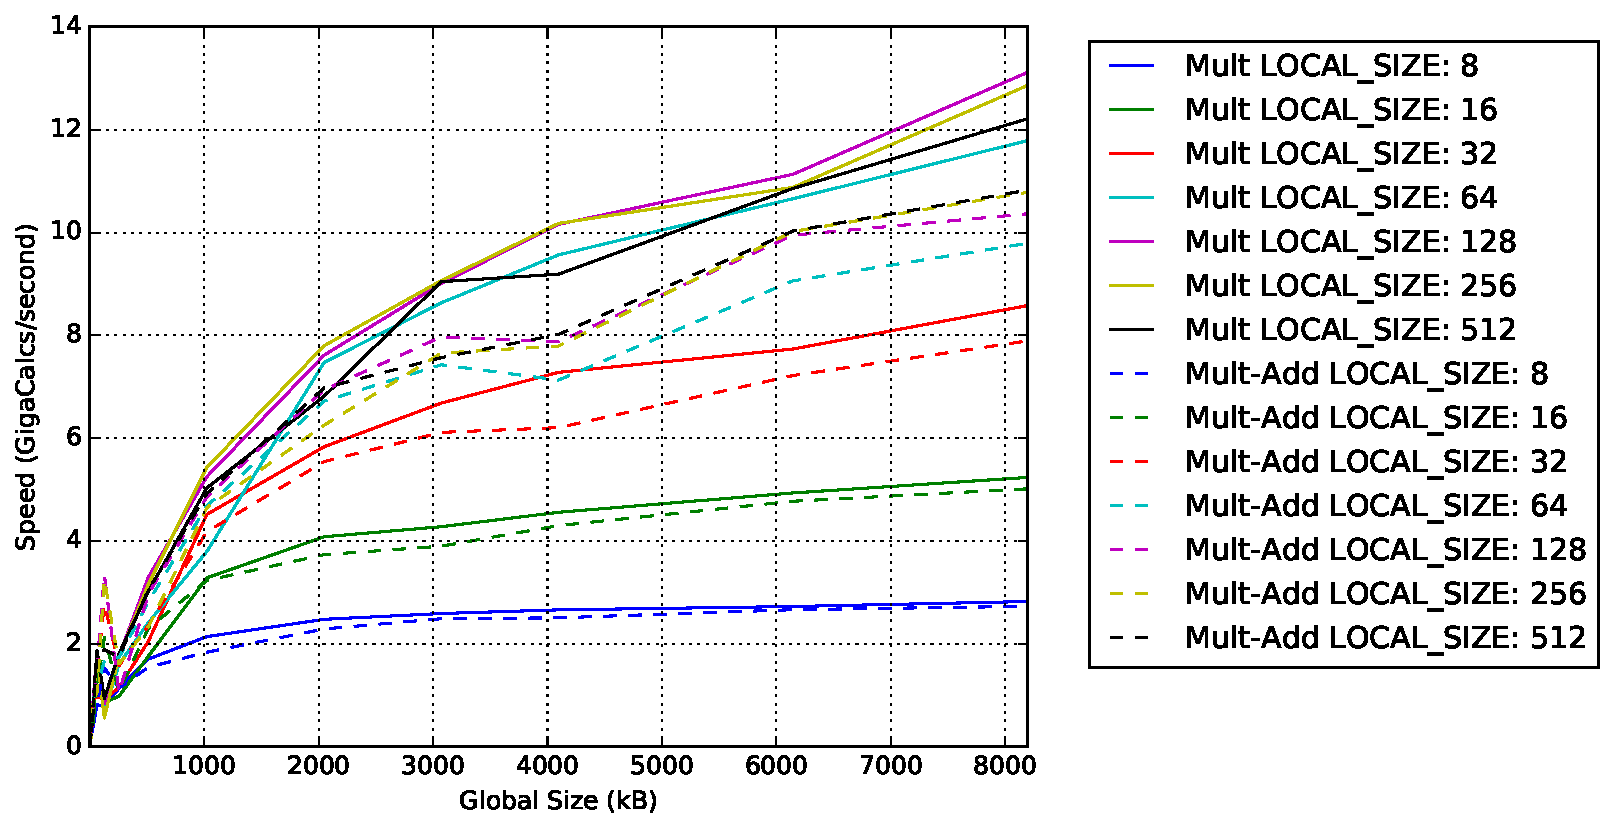
\includegraphics[width=0.65\linewidth]{Mult_Arraysize_2.pdf}
        \caption{Speed of the multiplication and multiplication with addition experiments vs. global size.  Note that the solid lines signify multiplication, while the dashed lines signify multiplication with addition.}
        \label{fig:MultGlobal}
\end{figure}
\begin{figure}[h!]
	\centering
        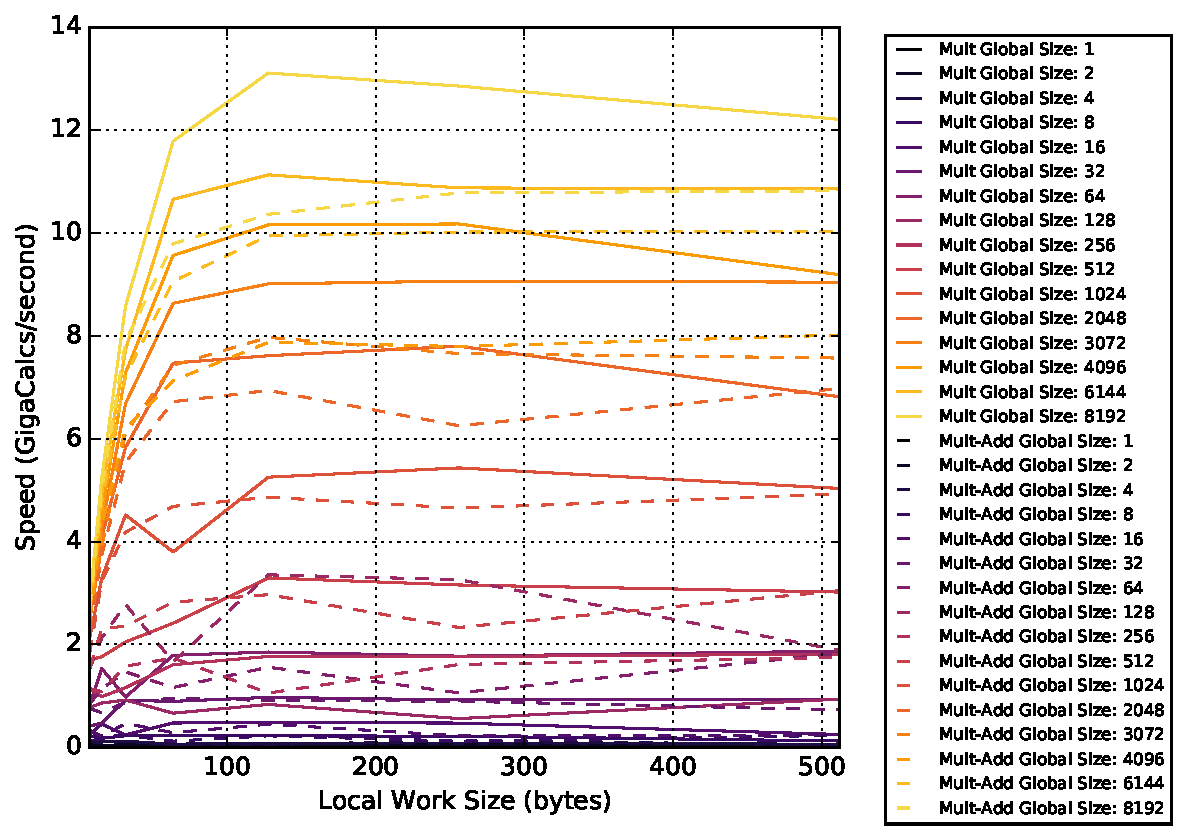
\includegraphics[width=0.65\linewidth]{Mult_Localsize_2.pdf}
        \caption{Speed of the multiplication and multiplication with addition experiments vs. local size.  Note that the solid lines signify multiplication, while the dashed lines signify multiplication with addition.}
        \label{fig:MultLocal}
\end{figure}

\newpage

\subsection*{Question 3}
\textit{What patterns are you seeing in the performance curves of array multiplication and array multiplication-addition?}

As seen in Figure \ref{fig:MultGlobal}, as the global work size increases, the performance increases for almost all values of the local work size.  For some values of the local work size, particularly smaller values (\texttt{LOCAL\_WORK\_SIZE} $< \sim 16$), the performance begins to hit a plateau as the global work size increased.  It is possible that with global work sizes much greater than 8MB, the performance will plateau for all of the larger values of \texttt{LOCAL\_WORK\_SIZE}.

As seen in Figure \ref{fig:MultLocal}, the performance is largely flat beyond a \texttt{LOCAL\_WORK\_SIZE} of approximately 128 bytes, and may slightly degrade beyond a \texttt{LOCAL\_WORK\_SIZE} of approximately 256.  Thus, there may be an optimal value of the local work size for each value of the global work size, however more testing would be needed to verify these results.

When either very small global work sizes or local work sizes were selected, performance was very poor.

\subsection*{Question 4}
\textit{Why do you think the patterns of array multiplication and array multiplication-addition look this way?}

The performance increases as the global work size increases because the experiment may be easily run in parallel.  There is a significant amount of computational overhead in setting up the problem to be run on a GPU versus a CPU, and therefore at small values of the global work size the parallelism is not worth the setup cost.  However, as the global work size gets bigger, the parallel fraction increases, making the problem more optimal for a GPU setup with OpenCL.

Having a local work size too small is not efficient because the GPU only has a limited number of processing elements, and with too small a work group each work group will be assigned a small amount of work at a given point in time.  It will therefore need to have have work reassigned to it often, which degrades performance.  With larger local work sizes, this will not be an issue.  Performance remains relatively flat as the local work size increases because the overhead becomes a relatively or even insignificantly small portion of the overall computational cost.  However, performance may begin to degrade as the local work size gets to be large due to issues storing large amounts of data in memory on the GPU.

\subsection*{Question 5}
\textit{What is the performance difference between doing a multiply and doing a multiply-add?}

The performance of multiplication was in all cases slightly greater than the performance of multiplication with addition for the same global work size and local work size.  The number of calculations per second does not take into account that multiplication operations consisted of only one calculation, while operations of multiplication with addition consisted of two calculations.  Thus, although the performance dropped slightly with multiplication with addition versus multiplication alone, the actual number of calculations per second may be greater due to the increased amount of work done.  This may be due to the increased amount of instructions associated with a similar overhead, or it may have to do with the fact that GPU hardware supports simultaneous multiplication and addition in some circumstances.

\subsection*{Question 6}
\textit{What does the difference in performance between doing a multiply and a multiply-add mean for the proper use of GPU parallel computing?}

Although multiplication alone is faster than multiplication with addition, the difference between the two is not huge.  Because multiplication with addition involves more computations than multiplication alone, it may be more efficient to do multiplication with addition than multiplication alone with addition separate, and the two should be done together whenever both operations are needed.

\newpage
\subsection*{Question 7}
\textit{Show a table and graph for the performance of the multiplication-reduction experiment.}

Graphs of the computation speed versus the global size and local work group size can be found in Figures \ref{fig:ReducGlobal} and \ref{fig:ReducLocal}.  A table of the values used to generate these graphs can be found along with the values for multiplication and multiplication with addition in Table \ref{tab:Data} of Appendix \ref{app:Data}.

\begin{figure}[h]
	\centering
        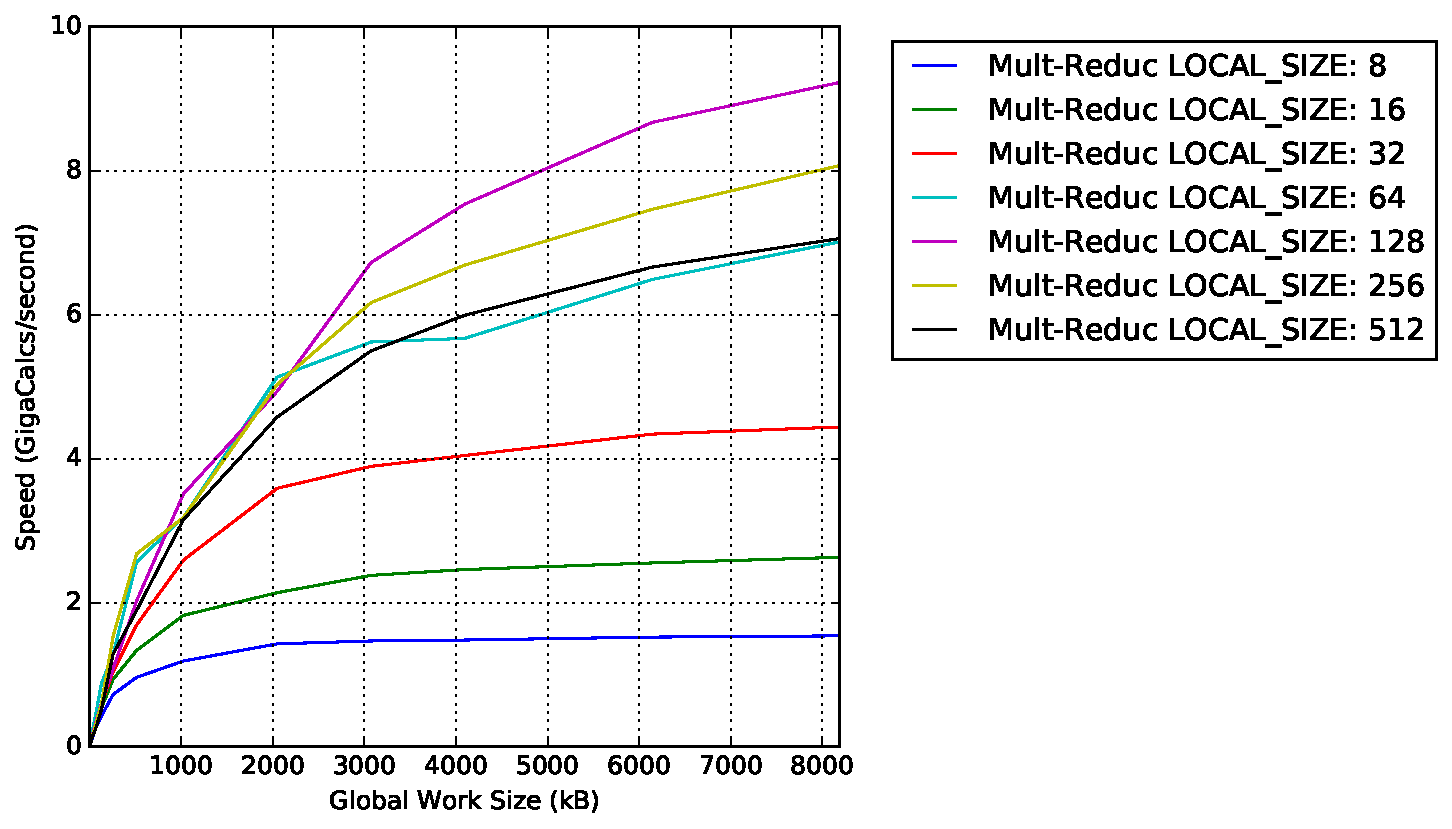
\includegraphics[width=0.7\linewidth]{Mult_Reduc_Arraysize_2.pdf}
        \caption{Speed of the multiplication with reduction experiment vs. global size.}
        \label{fig:ReducGlobal}
\end{figure}

\begin{figure}[h]
	\centering
        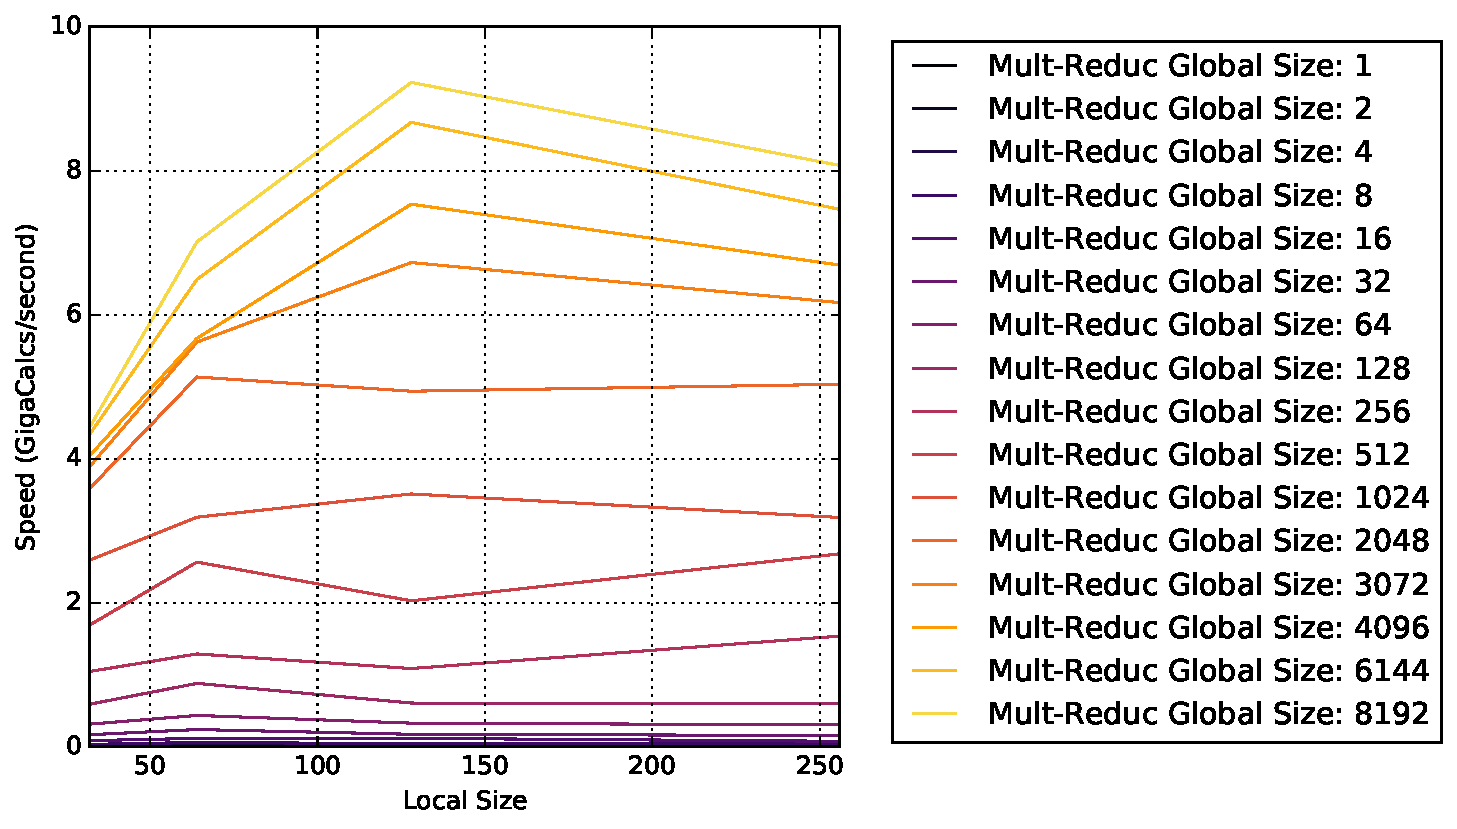
\includegraphics[width=0.7\linewidth]{Mult_Reduc_Localsize_2.pdf}
        \caption{Speed of the multiplication with reduction experiment vs. local size.}
        \label{fig:ReducLocal}
\end{figure}

\subsection*{Question 8}
\textit{What patterns are you seeing in the performance curves of the multiplication-reduction experiment?}

The performance curves of the multiplication with reduction in both Figures \ref{fig:ReducGlobal} and \ref{fig:ReducLocal} are largely similar to the curves seen earlier in Figures \ref{fig:MultGlobal} and \ref{fig:MultLocal}.  The performance appears to plateau slightly more with multiplication with reduction than it does for either multiplication or multiplication with addition as the global work size gets larger.

The performance of the multiplication-reduction experiment appears to peak more with a \texttt{LOCAL\_WORK\_SIZE} of 128 than it did with either the multiplication or the multiplication with addition experiments.

Overall, the performance of the multiplication-reduction experiment was overall similar to the performance of the multiplication with addition experiment.

\subsection*{Question 9}
\textit{Why do you think the patterns of the multiplication-reduction experiment look this way?}

The reasons that the patterns of the multiplication-reduction experiment look the way they do are similar to the reasons that the multiplication and multiplication with addition experiments exhibit the same trends.

The reasoning for the increased tendency of the multiplication-reduction experiment to plateau may be because the data eventually becomes less and less parallel as the reduction progresses.  With data that is not highly parallel, the performance of the GPU diminishes when compared to the performance of a CPU.

\subsection*{Question 10}
\textit{What do the patterns in the multiplication-reduction experiment mean for the proper use of GPU parallel computing?}

The GPU can be used to efficiently multiply and reduce a set of data.  The high performance of the operation means that with large sets of data to be handled in this manner, a GPU should be employed, with larger sets of data corresponding to an increase in performance.

\newpage
\section{Appendices}
\subsection{Tables of Generated Data}
\label{app:Data}

\begin{longtable}{|l|l|l|l|l|}
\caption{Raw Data Generated}\label{tab:Data}\\
\hline
Mode               & NKB  & LOCAL\_SIZE & NUM\_WORK\_GROUPS & GigaCalcPerSecond \\ \hline
Multiply           & 1    & 8           & 128               & 0.028             \\ \hline
Multiply           & 2    & 8           & 256               & 0.057             \\ \hline
Multiply           & 4    & 8           & 512               & 0.120             \\ \hline
Multiply           & 8    & 8           & 1024              & 0.118             \\ \hline
Multiply           & 16   & 8           & 2048              & 0.249             \\ \hline
Multiply           & 32   & 8           & 4096              & 0.414             \\ \hline
Multiply           & 64   & 8           & 8192              & 0.822             \\ \hline
Multiply           & 128  & 8           & 16384             & 0.777             \\ \hline
Multiply           & 256  & 8           & 32768             & 1.139             \\ \hline
Multiply           & 512  & 8           & 65536             & 1.705             \\ \hline
Multiply           & 1024 & 8           & 131072            & 2.143             \\ \hline
Multiply           & 2048 & 8           & 262144            & 2.479             \\ \hline
Multiply           & 3072 & 8           & 393216            & 2.592             \\ \hline
Multiply           & 4096 & 8           & 524288            & 2.663             \\ \hline
Multiply           & 6144 & 8           & 786432            & 2.728             \\ \hline
Multiply           & 8192 & 8           & 1048576           & 2.825             \\ \hline
Multiply           & 1    & 16          & 64                & 0.029             \\ \hline
Multiply           & 2    & 16          & 128               & 0.027             \\ \hline
Multiply           & 4    & 16          & 256               & 0.119             \\ \hline
Multiply           & 8    & 16          & 512               & 0.176             \\ \hline
Multiply           & 16   & 16          & 1024              & 0.452             \\ \hline
Multiply           & 32   & 16          & 2048              & 0.471             \\ \hline
Multiply           & 64   & 16          & 4096              & 1.532             \\ \hline
Multiply           & 128  & 16          & 8192              & 0.861             \\ \hline
Multiply           & 256  & 16          & 16384             & 0.985             \\ \hline
Multiply           & 512  & 16          & 32768             & 1.760             \\ \hline
Multiply           & 1024 & 16          & 65536             & 3.286             \\ \hline
Multiply           & 2048 & 16          & 131072            & 4.084             \\ \hline
Multiply           & 3072 & 16          & 196608            & 4.280             \\ \hline
Multiply           & 4096 & 16          & 262144            & 4.560             \\ \hline
Multiply           & 6144 & 16          & 393216            & 4.936             \\ \hline
Multiply           & 8192 & 16          & 524288            & 5.238             \\ \hline
Multiply           & 1    & 32          & 32                & 0.017             \\ \hline
Multiply           & 2    & 32          & 64                & 0.061             \\ \hline
Multiply           & 4    & 32          & 128               & 0.118             \\ \hline
Multiply           & 8    & 32          & 256               & 0.225             \\ \hline
Multiply           & 16   & 32          & 512               & 0.243             \\ \hline
Multiply           & 32   & 32          & 1024              & 0.914             \\ \hline
Multiply           & 64   & 32          & 2048              & 0.976             \\ \hline
Multiply           & 128  & 32          & 4096              & 0.920             \\ \hline
Multiply           & 256  & 32          & 8192              & 1.160             \\ \hline
Multiply           & 512  & 32          & 16384             & 2.048             \\ \hline
Multiply           & 1024 & 32          & 32768             & 4.519             \\ \hline
Multiply           & 2048 & 32          & 65536             & 5.834             \\ \hline
Multiply           & 3072 & 32          & 98304             & 6.684             \\ \hline
Multiply           & 4096 & 32          & 131072            & 7.281             \\ \hline
Multiply           & 6144 & 32          & 196608            & 7.735             \\ \hline
Multiply           & 8192 & 32          & 262144            & 8.579             \\ \hline
Multiply           & 1    & 64          & 16                & 0.030             \\ \hline
Multiply           & 2    & 64          & 32                & 0.061             \\ \hline
Multiply           & 4    & 64          & 64                & 0.061             \\ \hline
Multiply           & 8    & 64          & 128               & 0.232             \\ \hline
Multiply           & 16   & 64          & 256               & 0.473             \\ \hline
Multiply           & 32   & 64          & 512               & 0.894             \\ \hline
Multiply           & 64   & 64          & 1024              & 1.790             \\ \hline
Multiply           & 128  & 64          & 2048              & 0.664             \\ \hline
Multiply           & 256  & 64          & 4096              & 1.607             \\ \hline
Multiply           & 512  & 64          & 8192              & 2.413             \\ \hline
Multiply           & 1024 & 64          & 16384             & 3.799             \\ \hline
Multiply           & 2048 & 64          & 32768             & 7.471             \\ \hline
Multiply           & 3072 & 64          & 49152             & 8.634             \\ \hline
Multiply           & 4096 & 64          & 65536             & 9.565             \\ \hline
Multiply           & 6144 & 64          & 98304             & 10.657            \\ \hline
Multiply           & 8192 & 64          & 131072            & 11.786            \\ \hline
Multiply           & 1    & 128         & 8                 & 0.028             \\ \hline
Multiply           & 2    & 128         & 16                & 0.058             \\ \hline
Multiply           & 4    & 128         & 32                & 0.082             \\ \hline
Multiply           & 8    & 128         & 64                & 0.223             \\ \hline
Multiply           & 16   & 128         & 128               & 0.483             \\ \hline
Multiply           & 32   & 128         & 256               & 0.972             \\ \hline
Multiply           & 64   & 128         & 512               & 1.853             \\ \hline
Multiply           & 128  & 128         & 1024              & 0.834             \\ \hline
Multiply           & 256  & 128         & 2048              & 1.768             \\ \hline
Multiply           & 512  & 128         & 4096              & 3.294             \\ \hline
Multiply           & 1024 & 128         & 8192              & 5.253             \\ \hline
Multiply           & 2048 & 128         & 16384             & 7.615             \\ \hline
Multiply           & 3072 & 128         & 24576             & 9.012             \\ \hline
Multiply           & 4096 & 128         & 32768             & 10.159            \\ \hline
Multiply           & 6144 & 128         & 49152             & 11.132            \\ \hline
Multiply           & 8192 & 128         & 65536             & 13.112            \\ \hline
Multiply           & 1    & 256         & 4                 & 0.030             \\ \hline
Multiply           & 2    & 256         & 8                 & 0.060             \\ \hline
Multiply           & 4    & 256         & 16                & 0.082             \\ \hline
Multiply           & 8    & 256         & 32                & 0.217             \\ \hline
Multiply           & 16   & 256         & 64                & 0.472             \\ \hline
Multiply           & 32   & 256         & 128               & 0.921             \\ \hline
Multiply           & 64   & 256         & 256               & 1.773             \\ \hline
Multiply           & 128  & 256         & 512               & 0.559             \\ \hline
Multiply           & 256  & 256         & 1024              & 1.766             \\ \hline
Multiply           & 512  & 256         & 2048              & 3.157             \\ \hline
Multiply           & 1024 & 256         & 4096              & 5.433             \\ \hline
Multiply           & 2048 & 256         & 8192              & 7.799             \\ \hline
Multiply           & 3072 & 256         & 12288             & 9.065             \\ \hline
Multiply           & 4096 & 256         & 16384             & 10.177            \\ \hline
Multiply           & 6144 & 256         & 24576             & 10.878            \\ \hline
Multiply           & 8192 & 256         & 32768             & 12.858            \\ \hline
Multiply           & 1    & 512         & 2                 & 0.029             \\ \hline
Multiply           & 2    & 512         & 4                 & 0.059             \\ \hline
Multiply           & 4    & 512         & 8                 & 0.060             \\ \hline
Multiply           & 8    & 512         & 16                & 0.123             \\ \hline
Multiply           & 16   & 512         & 32                & 0.250             \\ \hline
Multiply           & 32   & 512         & 64                & 0.928             \\ \hline
Multiply           & 64   & 512         & 128               & 1.870             \\ \hline
Multiply           & 128  & 512         & 256               & 0.939             \\ \hline
Multiply           & 256  & 512         & 512               & 1.812             \\ \hline
Multiply           & 512  & 512         & 1024              & 3.019             \\ \hline
Multiply           & 1024 & 512         & 2048              & 5.034             \\ \hline
Multiply           & 2048 & 512         & 4096              & 6.816             \\ \hline
Multiply           & 3072 & 512         & 6144              & 9.045             \\ \hline
Multiply           & 4096 & 512         & 8192              & 9.190             \\ \hline
Multiply           & 6144 & 512         & 12288             & 10.857            \\ \hline
Multiply           & 8192 & 512         & 16384             & 12.210            \\ \hline
Multiply-Add       & 1    & 8           & 128               & 0.031             \\ \hline
Multiply-Add       & 2    & 8           & 256               & 0.057             \\ \hline
Multiply-Add       & 4    & 8           & 512               & 0.112             \\ \hline
Multiply-Add       & 8    & 8           & 1024              & 0.219             \\ \hline
Multiply-Add       & 16   & 8           & 2048              & 0.333             \\ \hline
Multiply-Add       & 32   & 8           & 4096              & 0.753             \\ \hline
Multiply-Add       & 64   & 8           & 8192              & 0.847             \\ \hline
Multiply-Add       & 128  & 8           & 16384             & 1.530             \\ \hline
Multiply-Add       & 256  & 8           & 32768             & 1.143             \\ \hline
Multiply-Add       & 512  & 8           & 65536             & 1.547             \\ \hline
Multiply-Add       & 1024 & 8           & 131072            & 1.840             \\ \hline
Multiply-Add       & 2048 & 8           & 262144            & 2.292             \\ \hline
Multiply-Add       & 3072 & 8           & 393216            & 2.492             \\ \hline
Multiply-Add       & 4096 & 8           & 524288            & 2.508             \\ \hline
Multiply-Add       & 6144 & 8           & 786432            & 2.667             \\ \hline
Multiply-Add       & 8192 & 8           & 1048576           & 2.732             \\ \hline
Multiply-Add       & 1    & 16          & 64                & 0.029             \\ \hline
Multiply-Add       & 2    & 16          & 128               & 0.049             \\ \hline
Multiply-Add       & 4    & 16          & 256               & 0.089             \\ \hline
Multiply-Add       & 8    & 16          & 512               & 0.221             \\ \hline
Multiply-Add       & 16   & 16          & 1024              & 0.209             \\ \hline
Multiply-Add       & 32   & 16          & 2048              & 0.673             \\ \hline
Multiply-Add       & 64   & 16          & 4096              & 1.136             \\ \hline
Multiply-Add       & 128  & 16          & 8192              & 2.126             \\ \hline
Multiply-Add       & 256  & 16          & 16384             & 1.085             \\ \hline
Multiply-Add       & 512  & 16          & 32768             & 2.304             \\ \hline
Multiply-Add       & 1024 & 16          & 65536             & 3.235             \\ \hline
Multiply-Add       & 2048 & 16          & 131072            & 3.737             \\ \hline
Multiply-Add       & 3072 & 16          & 196608            & 3.901             \\ \hline
Multiply-Add       & 4096 & 16          & 262144            & 4.302             \\ \hline
Multiply-Add       & 6144 & 16          & 393216            & 4.775             \\ \hline
Multiply-Add       & 8192 & 16          & 524288            & 5.017             \\ \hline
Multiply-Add       & 1    & 32          & 32                & 0.030             \\ \hline
Multiply-Add       & 2    & 32          & 64                & 0.030             \\ \hline
Multiply-Add       & 4    & 32          & 128               & 0.115             \\ \hline
Multiply-Add       & 8    & 32          & 256               & 0.234             \\ \hline
Multiply-Add       & 16   & 32          & 512               & 0.465             \\ \hline
Multiply-Add       & 32   & 32          & 1024              & 0.877             \\ \hline
Multiply-Add       & 64   & 32          & 2048              & 1.466             \\ \hline
Multiply-Add       & 128  & 32          & 4096              & 2.779             \\ \hline
Multiply-Add       & 256  & 32          & 8192              & 1.578             \\ \hline
Multiply-Add       & 512  & 32          & 16384             & 2.358             \\ \hline
Multiply-Add       & 1024 & 32          & 32768             & 4.183             \\ \hline
Multiply-Add       & 2048 & 32          & 65536             & 5.545             \\ \hline
Multiply-Add       & 3072 & 32          & 98304             & 6.114             \\ \hline
Multiply-Add       & 4096 & 32          & 131072            & 6.206             \\ \hline
Multiply-Add       & 6144 & 32          & 196608            & 7.219             \\ \hline
Multiply-Add       & 8192 & 32          & 262144            & 7.892             \\ \hline
Multiply-Add       & 1    & 64          & 16                & 0.015             \\ \hline
Multiply-Add       & 2    & 64          & 32                & 0.061             \\ \hline
Multiply-Add       & 4    & 64          & 64                & 0.058             \\ \hline
Multiply-Add       & 8    & 64          & 128               & 0.120             \\ \hline
Multiply-Add       & 16   & 64          & 256               & 0.284             \\ \hline
Multiply-Add       & 32   & 64          & 512               & 0.955             \\ \hline
Multiply-Add       & 64   & 64          & 1024              & 1.163             \\ \hline
Multiply-Add       & 128  & 64          & 2048              & 1.664             \\ \hline
Multiply-Add       & 256  & 64          & 4096              & 1.736             \\ \hline
Multiply-Add       & 512  & 64          & 8192              & 2.821             \\ \hline
Multiply-Add       & 1024 & 64          & 16384             & 4.685             \\ \hline
Multiply-Add       & 2048 & 64          & 32768             & 6.721             \\ \hline
Multiply-Add       & 3072 & 64          & 49152             & 7.428             \\ \hline
Multiply-Add       & 4096 & 64          & 65536             & 7.131             \\ \hline
Multiply-Add       & 6144 & 64          & 98304             & 9.060             \\ \hline
Multiply-Add       & 8192 & 64          & 131072            & 9.791             \\ \hline
Multiply-Add       & 1    & 128         & 8                 & 0.027             \\ \hline
Multiply-Add       & 2    & 128         & 16                & 0.057             \\ \hline
Multiply-Add       & 4    & 128         & 32                & 0.058             \\ \hline
Multiply-Add       & 8    & 128         & 64                & 0.224             \\ \hline
Multiply-Add       & 16   & 128         & 128               & 0.451             \\ \hline
Multiply-Add       & 32   & 128         & 256               & 0.911             \\ \hline
Multiply-Add       & 64   & 128         & 512               & 1.558             \\ \hline
Multiply-Add       & 128  & 128         & 1024              & 3.354             \\ \hline
Multiply-Add       & 256  & 128         & 2048              & 1.055             \\ \hline
Multiply-Add       & 512  & 128         & 4096              & 2.969             \\ \hline
Multiply-Add       & 1024 & 128         & 8192              & 4.863             \\ \hline
Multiply-Add       & 2048 & 128         & 16384             & 6.940             \\ \hline
Multiply-Add       & 3072 & 128         & 24576             & 7.972             \\ \hline
Multiply-Add       & 4096 & 128         & 32768             & 7.875             \\ \hline
Multiply-Add       & 6144 & 128         & 49152             & 9.948             \\ \hline
Multiply-Add       & 8192 & 128         & 65536             & 10.364            \\ \hline
Multiply-Add       & 1    & 256         & 4                 & 0.030             \\ \hline
Multiply-Add       & 2    & 256         & 8                 & 0.059             \\ \hline
Multiply-Add       & 4    & 256         & 16                & 0.119             \\ \hline
Multiply-Add       & 8    & 256         & 32                & 0.120             \\ \hline
Multiply-Add       & 16   & 256         & 64                & 0.222             \\ \hline
Multiply-Add       & 32   & 256         & 128               & 0.898             \\ \hline
Multiply-Add       & 64   & 256         & 256               & 1.059             \\ \hline
Multiply-Add       & 128  & 256         & 512               & 3.261             \\ \hline
Multiply-Add       & 256  & 256         & 1024              & 1.612             \\ \hline
Multiply-Add       & 512  & 256         & 2048              & 2.331             \\ \hline
Multiply-Add       & 1024 & 256         & 4096              & 4.651             \\ \hline
Multiply-Add       & 2048 & 256         & 8192              & 6.253             \\ \hline
Multiply-Add       & 3072 & 256         & 12288             & 7.655             \\ \hline
Multiply-Add       & 4096 & 256         & 16384             & 7.793             \\ \hline
Multiply-Add       & 6144 & 256         & 24576             & 10.020            \\ \hline
Multiply-Add       & 8192 & 256         & 32768             & 10.782            \\ \hline
Multiply-Add       & 1    & 512         & 2                 & 0.031             \\ \hline
Multiply-Add       & 2    & 512         & 4                 & 0.059             \\ \hline
Multiply-Add       & 4    & 512         & 8                 & 0.053             \\ \hline
Multiply-Add       & 8    & 512         & 16                & 0.235             \\ \hline
Multiply-Add       & 16   & 512         & 32                & 0.243             \\ \hline
Multiply-Add       & 32   & 512         & 64                & 0.727             \\ \hline
Multiply-Add       & 64   & 512         & 128               & 1.832             \\ \hline
Multiply-Add       & 128  & 512         & 256               & 1.888             \\ \hline
Multiply-Add       & 256  & 512         & 512               & 1.748             \\ \hline
Multiply-Add       & 512  & 512         & 1024              & 3.048             \\ \hline
Multiply-Add       & 1024 & 512         & 2048              & 4.926             \\ \hline
Multiply-Add       & 2048 & 512         & 4096              & 6.979             \\ \hline
Multiply-Add       & 3072 & 512         & 6144              & 7.568             \\ \hline
Multiply-Add       & 4096 & 512         & 8192              & 8.018             \\ \hline
Multiply-Add       & 6144 & 512         & 12288             & 10.029            \\ \hline
Multiply-Add       & 8192 & 512         & 16384             & 10.823            \\ \hline
Multiply+Reduction & 1    & 8           & 128               & 0.005             \\ \hline
Multiply+Reduction & 2    & 8           & 256               & 0.011             \\ \hline
Multiply+Reduction & 4    & 8           & 512               & 0.018             \\ \hline
Multiply+Reduction & 8    & 8           & 1024              & 0.035             \\ \hline
Multiply+Reduction & 16   & 8           & 2048              & 0.075             \\ \hline
Multiply+Reduction & 32   & 8           & 4096              & 0.138             \\ \hline
Multiply+Reduction & 64   & 8           & 8192              & 0.260             \\ \hline
Multiply+Reduction & 128  & 8           & 16384             & 0.430             \\ \hline
Multiply+Reduction & 256  & 8           & 32768             & 0.727             \\ \hline
Multiply+Reduction & 512  & 8           & 65536             & 0.965             \\ \hline
Multiply+Reduction & 1024 & 8           & 131072            & 1.192             \\ \hline
Multiply+Reduction & 2048 & 8           & 262144            & 1.430             \\ \hline
Multiply+Reduction & 3072 & 8           & 393216            & 1.470             \\ \hline
Multiply+Reduction & 4096 & 8           & 524288            & 1.483             \\ \hline
Multiply+Reduction & 6144 & 8           & 786432            & 1.524             \\ \hline
Multiply+Reduction & 8192 & 8           & 1048576           & 1.541             \\ \hline
Multiply+Reduction & 1    & 16          & 64                & 0.005             \\ \hline
Multiply+Reduction & 2    & 16          & 128               & 0.010             \\ \hline
Multiply+Reduction & 4    & 16          & 256               & 0.020             \\ \hline
Multiply+Reduction & 8    & 16          & 512               & 0.038             \\ \hline
Multiply+Reduction & 16   & 16          & 1024              & 0.083             \\ \hline
Multiply+Reduction & 32   & 16          & 2048              & 0.156             \\ \hline
Multiply+Reduction & 64   & 16          & 4096              & 0.281             \\ \hline
Multiply+Reduction & 128  & 16          & 8192              & 0.540             \\ \hline
Multiply+Reduction & 256  & 16          & 16384             & 0.938             \\ \hline
Multiply+Reduction & 512  & 16          & 32768             & 1.339             \\ \hline
Multiply+Reduction & 1024 & 16          & 65536             & 1.826             \\ \hline
Multiply+Reduction & 2048 & 16          & 131072            & 2.141             \\ \hline
Multiply+Reduction & 3072 & 16          & 196608            & 2.381             \\ \hline
Multiply+Reduction & 4096 & 16          & 262144            & 2.462             \\ \hline
Multiply+Reduction & 6144 & 16          & 393216            & 2.554             \\ \hline
Multiply+Reduction & 8192 & 16          & 524288            & 2.632             \\ \hline
Multiply+Reduction & 1    & 32          & 32                & 0.005             \\ \hline
Multiply+Reduction & 2    & 32          & 64                & 0.010             \\ \hline
Multiply+Reduction & 4    & 32          & 128               & 0.022             \\ \hline
Multiply+Reduction & 8    & 32          & 256               & 0.034             \\ \hline
Multiply+Reduction & 16   & 32          & 512               & 0.086             \\ \hline
Multiply+Reduction & 32   & 32          & 1024              & 0.168             \\ \hline
Multiply+Reduction & 64   & 32          & 2048              & 0.315             \\ \hline
Multiply+Reduction & 128  & 32          & 4096              & 0.592             \\ \hline
Multiply+Reduction & 256  & 32          & 8192              & 1.047             \\ \hline
Multiply+Reduction & 512  & 32          & 16384             & 1.692             \\ \hline
Multiply+Reduction & 1024 & 32          & 32768             & 2.594             \\ \hline
Multiply+Reduction & 2048 & 32          & 65536             & 3.591             \\ \hline
Multiply+Reduction & 3072 & 32          & 98304             & 3.895             \\ \hline
Multiply+Reduction & 4096 & 32          & 131072            & 4.046             \\ \hline
Multiply+Reduction & 6144 & 32          & 196608            & 4.343             \\ \hline
Multiply+Reduction & 8192 & 32          & 262144            & 4.442             \\ \hline
Multiply+Reduction & 1    & 64          & 16                & 0.005             \\ \hline
Multiply+Reduction & 2    & 64          & 32                & 0.015             \\ \hline
Multiply+Reduction & 4    & 64          & 64                & 0.027             \\ \hline
Multiply+Reduction & 8    & 64          & 128               & 0.060             \\ \hline
Multiply+Reduction & 16   & 64          & 256               & 0.117             \\ \hline
Multiply+Reduction & 32   & 64          & 512               & 0.240             \\ \hline
Multiply+Reduction & 64   & 64          & 1024              & 0.436             \\ \hline
Multiply+Reduction & 128  & 64          & 2048              & 0.881             \\ \hline
Multiply+Reduction & 256  & 64          & 4096              & 1.290             \\ \hline
Multiply+Reduction & 512  & 64          & 8192              & 2.566             \\ \hline
Multiply+Reduction & 1024 & 64          & 16384             & 3.189             \\ \hline
Multiply+Reduction & 2048 & 64          & 32768             & 5.136             \\ \hline
Multiply+Reduction & 3072 & 64          & 49152             & 5.622             \\ \hline
Multiply+Reduction & 4096 & 64          & 65536             & 5.673             \\ \hline
Multiply+Reduction & 6144 & 64          & 98304             & 6.491             \\ \hline
Multiply+Reduction & 8192 & 64          & 131072            & 7.014             \\ \hline
Multiply+Reduction & 1    & 128         & 8                 & 0.005             \\ \hline
Multiply+Reduction & 2    & 128         & 16                & 0.014             \\ \hline
Multiply+Reduction & 4    & 128         & 32                & 0.031             \\ \hline
Multiply+Reduction & 8    & 128         & 64                & 0.044             \\ \hline
Multiply+Reduction & 16   & 128         & 128               & 0.118             \\ \hline
Multiply+Reduction & 32   & 128         & 256               & 0.174             \\ \hline
Multiply+Reduction & 64   & 128         & 512               & 0.329             \\ \hline
Multiply+Reduction & 128  & 128         & 1024              & 0.608             \\ \hline
Multiply+Reduction & 256  & 128         & 2048              & 1.087             \\ \hline
Multiply+Reduction & 512  & 128         & 4096              & 2.028             \\ \hline
Multiply+Reduction & 1024 & 128         & 8192              & 3.512             \\ \hline
Multiply+Reduction & 2048 & 128         & 16384             & 4.939             \\ \hline
Multiply+Reduction & 3072 & 128         & 24576             & 6.726             \\ \hline
Multiply+Reduction & 4096 & 128         & 32768             & 7.537             \\ \hline
Multiply+Reduction & 6144 & 128         & 49152             & 8.673             \\ \hline
Multiply+Reduction & 8192 & 128         & 65536             & 9.228             \\ \hline
Multiply+Reduction & 1    & 256         & 4                 & 0.005             \\ \hline
Multiply+Reduction & 2    & 256         & 8                 & 0.009             \\ \hline
Multiply+Reduction & 4    & 256         & 16                & 0.018             \\ \hline
Multiply+Reduction & 8    & 256         & 32                & 0.039             \\ \hline
Multiply+Reduction & 16   & 256         & 64                & 0.077             \\ \hline
Multiply+Reduction & 32   & 256         & 128               & 0.157             \\ \hline
Multiply+Reduction & 64   & 256         & 256               & 0.304             \\ \hline
Multiply+Reduction & 128  & 256         & 512               & 0.598             \\ \hline
Multiply+Reduction & 256  & 256         & 1024              & 1.538             \\ \hline
Multiply+Reduction & 512  & 256         & 2048              & 2.681             \\ \hline
Multiply+Reduction & 1024 & 256         & 4096              & 3.185             \\ \hline
Multiply+Reduction & 2048 & 256         & 8192              & 5.035             \\ \hline
Multiply+Reduction & 3072 & 256         & 12288             & 6.169             \\ \hline
Multiply+Reduction & 4096 & 256         & 16384             & 6.691             \\ \hline
Multiply+Reduction & 6144 & 256         & 24576             & 7.465             \\ \hline
Multiply+Reduction & 8192 & 256         & 32768             & 8.074             \\ \hline
Multiply+Reduction & 1    & 512         & 2                 & 0.005             \\ \hline
Multiply+Reduction & 2    & 512         & 4                 & 0.010             \\ \hline
Multiply+Reduction & 4    & 512         & 8                 & 0.020             \\ \hline
Multiply+Reduction & 8    & 512         & 16                & 0.038             \\ \hline
Multiply+Reduction & 16   & 512         & 32                & 0.077             \\ \hline
Multiply+Reduction & 32   & 512         & 64                & 0.149             \\ \hline
Multiply+Reduction & 64   & 512         & 128               & 0.246             \\ \hline
Multiply+Reduction & 128  & 512         & 256               & 0.517             \\ \hline
Multiply+Reduction & 256  & 512         & 512               & 1.290             \\ \hline
Multiply+Reduction & 512  & 512         & 1024              & 1.894             \\ \hline
Multiply+Reduction & 1024 & 512         & 2048              & 3.156             \\ \hline
Multiply+Reduction & 2048 & 512         & 4096              & 4.581             \\ \hline
Multiply+Reduction & 3072 & 512         & 6144              & 5.499             \\ \hline
Multiply+Reduction & 4096 & 512         & 8192              & 5.994             \\ \hline
Multiply+Reduction & 6144 & 512         & 12288             & 6.663             \\ \hline
Multiply+Reduction & 8192 & 512         & 16384             & 7.060             \\ \hline
\end{longtable}

\end{document}
